\hypertarget{digital-signal-processing-dsp---session-5}{%
\section{Digital Signal Processing (DSP) - Session
5}\label{digital-signal-processing-dsp---session-5}}

\begin{center}\rule{0.5\linewidth}{0.5pt}\end{center}

\hypertarget{plot-the-graph-of-xz-for-the-z-transform-with-python-and-matplotlib}{%
\subsection{\texorpdfstring{Plot the Graph of \(|X(z)|\) for the
z-transform with Python and
matplotlib}{Plot the Graph of \textbar X(z)\textbar{} for the z-transform with Python and matplotlib}}\label{plot-the-graph-of-xz-for-the-z-transform-with-python-and-matplotlib}}

\(|X(z)|\), the magnitude of \(X(z)\), is a real and positive function
of \(z\). Since \(z\) represents a point in the complex plane,
\(|X(z)|\) is a two-dimensional function and describes a ``surface.''

For example, plot the graph of \(|X(z)|\) for the z-transform

\[
X(z) = \frac{z^{-1} - z^{-2}}{1 - 1.2732z^{-1} + 0.81z^{-2}}
= \frac{z - 1}{z^2 - 1.2732z + 0.81}
\]

which has one zero at \(z_1 = 1\) and two poles at
\(p_1 = 0.9e^{j π/4}, p_2 = 0.9e^{-j π/4}\).

Reference: https://matplotlib.org/stable/gallery/mplot3d/subplot3d.html

\begin{Shaded}
\begin{Highlighting}[]
\ImportTok{import}\NormalTok{ matplotlib.pyplot }\ImportTok{as}\NormalTok{ plt}
\ImportTok{import}\NormalTok{ numpy }\ImportTok{as}\NormalTok{ np}
\ImportTok{from}\NormalTok{ matplotlib }\ImportTok{import}\NormalTok{ cm}

\CommentTok{\# set up a figure twice as wide as it is tall}
\NormalTok{fig }\OperatorTok{=}\NormalTok{ plt.figure(figsize}\OperatorTok{=}\NormalTok{plt.figaspect(}\FloatTok{0.5}\NormalTok{))}

\CommentTok{\# set up the Axes}
\NormalTok{ax }\OperatorTok{=}\NormalTok{ fig.add\_subplot(}\DecValTok{1}\NormalTok{, }\DecValTok{1}\NormalTok{, }\DecValTok{1}\NormalTok{, projection}\OperatorTok{=}\StringTok{\textquotesingle{}3d\textquotesingle{}}\NormalTok{)}

\CommentTok{\# plot a 3D surface like in the example mplot3d/surface3d\_demo}
\NormalTok{X }\OperatorTok{=}\NormalTok{ np.arange(}\OperatorTok{{-}}\DecValTok{5}\NormalTok{, }\DecValTok{5}\NormalTok{, }\FloatTok{0.1}\NormalTok{)}
\NormalTok{Y }\OperatorTok{=}\NormalTok{ np.arange(}\OperatorTok{{-}}\DecValTok{5}\NormalTok{, }\DecValTok{5}\NormalTok{, }\FloatTok{0.1}\NormalTok{)}
\NormalTok{X, Y }\OperatorTok{=}\NormalTok{ np.meshgrid(X, Y)}
\NormalTok{H }\OperatorTok{=}\NormalTok{ X}\OperatorTok{+}\NormalTok{Y}\OperatorTok{*}\OtherTok{1j}
\NormalTok{Z }\OperatorTok{=}\NormalTok{ np.}\BuiltInTok{abs}\NormalTok{((H}\OperatorTok{**{-}}\DecValTok{1}\OperatorTok{{-}}\NormalTok{H}\OperatorTok{**{-}}\DecValTok{2}\NormalTok{)}\OperatorTok{/}\NormalTok{(}\DecValTok{1}\OperatorTok{{-}}\FloatTok{1.2732}\OperatorTok{*}\NormalTok{H}\OperatorTok{**{-}}\DecValTok{1}\OperatorTok{+}\FloatTok{0.81}\OperatorTok{*}\NormalTok{H}\OperatorTok{**{-}}\DecValTok{2}\NormalTok{))}
\NormalTok{surf }\OperatorTok{=}\NormalTok{ ax.plot\_surface(X, Y, Z, rstride}\OperatorTok{=}\DecValTok{1}\NormalTok{, cstride}\OperatorTok{=}\DecValTok{1}\NormalTok{, cmap}\OperatorTok{=}\NormalTok{cm.coolwarm,}
\NormalTok{linewidth}\OperatorTok{=}\DecValTok{0}\NormalTok{, antialiased}\OperatorTok{=}\VariableTok{False}\NormalTok{)}
\NormalTok{ax.set\_zlim(}\OperatorTok{{-}}\DecValTok{1}\NormalTok{, }\DecValTok{10}\NormalTok{)}
\NormalTok{fig.colorbar(surf, shrink}\OperatorTok{=}\FloatTok{0.5}\NormalTok{, aspect}\OperatorTok{=}\DecValTok{10}\NormalTok{)}
\end{Highlighting}
\end{Shaded}

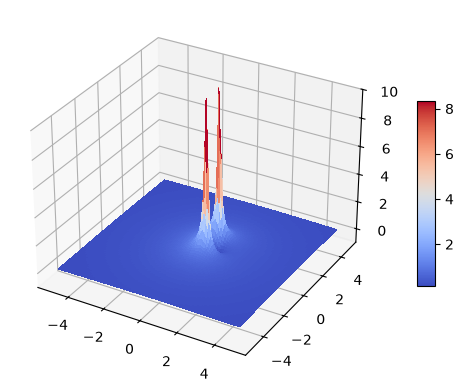
\includegraphics{z-transform-graph.png}

Note the high peaks near the singularities (poles) and the deep valley
close to the zero.

\begin{center}\rule{0.5\linewidth}{0.5pt}\end{center}

\hypertarget{frequency-analysis-of-signals}{%
\subsection{Frequency Analysis of
Signals}\label{frequency-analysis-of-signals}}

\textbf{Frequency Analysis} involves decomposing a signal into its
frequency (sinusoidal) components to provide a mathematical and
pictorial representation of its frequency content, often called its
\textbf{spectrum}. This spectrum acts as a ``signature'' for the signal,
as different signal waveforms have different spectra.

\textbf{The Prism Analogy}: As a glass prism causes a beam of sunlight
to refract into a spectrum of colors, frequency analysis tools (like the
Fourier series or transform) analyze time-domain waveforms into their
component frequencies. Recombining these components to reconstruct the
original signal is a process known as \textbf{Fourier synthesis}.

\textbf{Importance for LTI Systems}: Decomposing signals into sinusoids
(or complex exponentials) is essential because when a sinusoid is passed
through a \textbf{Linear Time-Invariant (LTI) system}, the output is a
sinusoid of the same frequency, differing only in amplitude and phase.

We consider four cases based on whether the time variable is
\textbf{continuous or discrete} and whether the signal is
\textbf{periodic or aperiodic}:

\begin{enumerate}
\def\labelenumi{\arabic{enumi}.}
\tightlist
\item
  Continuous-Time Periodic Signals
\item
  Continuous-Time Aperiodic Signals
\item
  Discrete-Time Periodic Signals
\item
  Discrete-Time Aperiodic Signals
\end{enumerate}

\hypertarget{the-fourier-series-for-continuous-time-periodic-signals}{%
\subsubsection{The Fourier Series for Continuous-Time Periodic
Signals}\label{the-fourier-series-for-continuous-time-periodic-signals}}

The Fourier series is a mathematical representation used to decompose a
continuous-time periodic signal into a linear weighted sum of
harmonically related complex exponentials or sinusoids.

\textbf{Synthesis Equation}

\[x(t) = \sum_{k=-\infty}^{\infty} c_k e^{j2\pi k F_0 t}\]

This equation, called the \textbf{Fourier Series}, shows how a periodic
signal \(x(t)\) is constructed (synthesized) from its basic ``building
blocks''. These blocks are exponential signals \({e^{j2\pi k F_0 t}}\)
where \(k\) ranges from \(-\infty\) to \(\infty\). \(F_0\) represents
the \textbf{fundamental frequency}, which is the reciprocal of the
fundamental period \(T_p\) (\(F_0 = 1/T_p\)). The coefficients \(c_k\)
act as weighting factors that specify the shape of the resulting
waveform.

\textbf{Analysis Equation}

\[c_k = \frac{1}{T_p} \int_{T_p} x(t) e^{-j2\pi k F_0 t} dt\]

This equation is used to determine the \textbf{Fourier coefficients}
\(c_k\) from a given periodic signal \(x(t)\). The integration is
performed over any single period of length \(T_p\). Physically, each
\(c_k\) represents the amplitude and phase associated with the \(k\)-th
harmonic component of the signal. \(c_k\) is also used as features in
Machine Learning models.

\textbf{Key Spectral Representations}

The information contained in the complex-valued Fourier coefficients
\({c_k}\) can be visualized through different types of spectra:

\begin{itemize}
\tightlist
\item
  \textbf{Amplitude (Magnitude) Spectrum:} This is a plot of the
  magnitude of the coefficients, \({|c_k|}\), against the frequency
  \(kF_0\). It represents the ``strength'' of each harmonic component.
  For real-valued signals, this spectrum is always a \textbf{symmetric
  (even) function}.
\item
  \textbf{Phase Spectrum:} This is a plot of the phase angles,
  \({\theta_k = \angle c_k}\), against frequency. It represents the
  relative time-shift of each harmonic. For real-valued signals, the
  phase spectrum is an \textbf{antisymmetric (odd) function}.
\item
  \textbf{Power Density Spectrum:} This diagram plots \({|c_k|^2}\) as a
  function of frequency, showing how the total average power of the
  periodic signal is distributed among its various frequency components.
  Because power only exists at discrete values (multiples of \(F_0\)),
  it is often called a \textbf{line spectrum}.
\end{itemize}

\textbf{Key Properties}

\begin{itemize}
\tightlist
\item
  \textbf{Line Spectrum Characteristic:} Periodic signals possess
  discrete spectra where the spectral lines are equally spaced by the
  fundamental frequency \(F_0\).
\item
  \textbf{Symmetry for Real Signals:} If the signal \(x(t)\) is real,
  then \(c_{-k} = c_k^*\) (complex conjugates). This implies that the
  magnitude spectrum is even (\(|c_k| = |c_{-k}|\)) and the phase
  spectrum is odd (\(\theta_k = -\theta_{-k}\)).
\item
  \textbf{Parseval's Relation for Power Signals:} The total average
  power \(P_x\) of a periodic signal can be calculated by summing the
  power of all its individual harmonic components:
  \[P_x = \frac{1}{T_p} \int_{T_p} |x(t)|^2 dt = \sum_{k=-\infty}^{\infty} |c_k|^2\]
  This establishes the principle of \textbf{conservation of energy}
  between the time and frequency domains.
\end{itemize}

\textbf{Convergence and Dirichlet Conditions}

For the Fourier series to exactly equal \(x(t)\) at every value of
\(t\), the signal must satisfy the \textbf{Dirichlet conditions}:

\begin{enumerate}
\def\labelenumi{\arabic{enumi}.}
\tightlist
\item
  The signal \(x(t)\) must have a finite number of discontinuities
  within any period.
\item
  The signal \(x(t)\) must contain a finite number of maxima and minima
  during any period.
\item
  The signal \(x(t)\) must be absolutely integrable over a period. All
  periodic signals of practical interest generally satisfy these
  conditions.
\end{enumerate}

\begin{quote}
\textbf{\emph{Example 1.1}}

\textbf{Determine the Fourier series and the power density spectrum} of
the rectangular pulse train signal \(x(t)\) with amplitude \(A\) and
pulse width \(\tau\), periodic with fundamental period \(T_p\), as
illustrated in Fig 1.3.

\emph{Solution}

\begin{enumerate}
\def\labelenumi{\arabic{enumi}.}
\item
  \textbf{Identify Signal Properties:} The signal \(x(t)\) is periodic
  with fundamental period \(T_p\) and fundamental frequency
  \(F_0 = 1/T_p\). It is an \textbf{even signal} \(x(t) = x(-t)\), so it
  is convenient to integrate over the interval \([-T_p/2, T_p/2]\).
\item
  \textbf{Apply the Fourier Analysis Equation:} The Fourier coefficients
  \(c_k\) are determined using the analysis equation:
  \[c_k = \frac{1}{T_p} \int_{-T_p/2}^{T_p/2} x(t)e^{-j2\pi kF_0t} dt\]
\item
  \textbf{Determine \(c_0\) (DC Component):} For \(k=0\), the
  coefficient represents the average value of the signal over one
  period:
  \[c_0 = \frac{1}{T_p} \int_{-T_p/2}^{T_p/2} x(t) dt = \frac{1}{T_p} \int_{-\tau/2}^{\tau/2} A dt = \frac{A\tau}{T_p}\]
\item
  \textbf{Determine \(c_k\) for \(k \neq 0\):} Substitute the signal
  definition into the analysis equation:
  \[c_k = \frac{1}{T_p} \int_{-\tau/2}^{\tau/2} Ae^{-j2\pi kF_0t} dt\]
  \[c_k = \frac{A}{T_p} \left[ \frac{e^{-j2\pi kF_0t}}{-j2\pi kF_0} \right]_{-\tau/2}^{\tau/2}\]
  \[c_k = \frac{A}{-j2\pi kF_0T_p} (e^{-j\pi kF_0\tau} - e^{j\pi kF_0\tau})\]
\item
  \textbf{Simplify Using Euler's Identity:} Rearrange the terms to form
  the sine function, noting that \(F_0T_p = 1\):
  \[c_k = \frac{A}{\pi k} \left( \frac{e^{j\pi kF_0\tau} - e^{-j\pi kF_0\tau}}{j2} \right)\]
  \[c_k = \frac{A\tau}{T_p} \frac{\sin(\pi kF_0\tau)}{\pi kF_0\tau}, \quad k = \pm 1, \pm 2, \dots\]
  The coefficients are real-valued and takes the form of the sinc
  function \(\text{sinc}(\phi) = \frac{\sin (\phi)}{\phi}\) with zero
  crossings at \(kF_0 = m/\tau\).
\item
  \textbf{Determine the Power Density Spectrum} The power density
  spectrum \(|c_k|^2\) represents the power distribution across discrete
  frequencies \(kF_0\):
  \[|c_k|^2 = \begin{cases} \left( \frac{A\tau}{T_p} \right)^2, & k = 0 \\ \left( \frac{A\tau}{T_p} \right)^2 \left( \frac{\sin(\pi kF_0\tau)}{\pi kF_0\tau} \right)^2, & k = \pm 1, \pm 2, \dots \end{cases}\]
\end{enumerate}
\end{quote}

\hypertarget{the-fourier-transform-for-continuous-time-aperiodic-signals}{%
\subsubsection{The Fourier Transform for Continuous-Time Aperiodic
Signals}\label{the-fourier-transform-for-continuous-time-aperiodic-signals}}

The Fourier transform is a mathematical tool used to represent aperiodic
(non-periodic), finite-energy signals in the frequency domain. Unlike
periodic signals, which have discrete ``line'' spectra, aperiodic
signals possess a \textbf{continuous spectrum}.

\textbf{Synthesis Equation (Inverse Transform)}

\[x(t) = \int_{-\infty}^{\infty} X(F) e^{j2\pi Ft} dF\]

This equation describes the \textbf{synthesis} problem: how an aperiodic
signal \(x(t)\) is reconstructed from its frequency components. Because
the signal is not periodic, its frequency content is not limited to
discrete harmonics; instead, it is composed of a \textbf{continuum of
infinitesimal complex exponentials} \({e^{j2\pi Ft}}\). Consequently,
the reconstruction is performed through \textbf{integration} over all
frequencies from \(-\infty\) to \(\infty\) rather than a summation.

\textbf{Analysis Equation (Direct Transform)}

\[X(F) = \int_{-\infty}^{\infty} x(t) e^{-j2\pi Ft} dt\]

This equation, called the \textbf{Fourier Transform}, is used for
\textbf{spectral analysis}. It determines the function \(X(F)\), which
represents the \textbf{frequency content} of the signal \(x(t)\).
Physically, \(X(F)\) acts as a ``signature'' for the signal, providing a
mathematical and pictorial representation of its frequency components.

\textbf{Key Spectral Representations}

The complex-valued function \(X(F)\) is typically expressed in polar
form to visualize the signal's characteristics:

\begin{itemize}
\tightlist
\item
  \textbf{Amplitude (Magnitude) Spectrum:} Denoted as
  \textbf{\(|X(F)|\)}, this represents the distribution of the
  magnitudes of the frequency components. For real-valued signals, this
  spectrum exhibits \textbf{even symmetry} (\(|X(F)| = |X(-F)|\)).
\item
  \textbf{Phase Spectrum:} Denoted as \textbf{\(\theta(F)\)} or
  \textbf{\(\angle X(F)\)}, this represents the phase shift associated
  with each frequency. For real signals, the phase spectrum has
  \textbf{odd symmetry} (\(\angle X(-F) = -\angle X(F)\)).
\item
  \textbf{Energy Density Spectrum:} Defined as
  \textbf{\(S_{xx}(F) = |X(F)|^2\)}, this function describes how the
  total energy of a signal is distributed across different frequencies.
  It contains no phase information and is always purely real and
  non-negative.
\end{itemize}

\textbf{Key Properties}

\begin{itemize}
\tightlist
\item
  \textbf{Continuous Spectrum:} Because aperiodic signals have an
  infinite period (\(T_p \to \infty\)), the spacing between spectral
  lines in a periodic representation tends toward zero, resulting in a
  continuous frequency range.
\item
  \textbf{Uncertainty Principle:} There is an inverse relationship
  between a signal's duration in time and its bandwidth in frequency;
  for example, if a signal is compressed (shortened) in time, its
  Fourier transform is expanded (widened) in frequency.
\item
  \textbf{Parseval's Relation for Energy Signals:} The total energy
  \(E_x\) of the signal can be calculated in either the time or
  frequency domain:
  \[E_x = \int_{-\infty}^{\infty} |x(t)|^2 dt = \int_{-\infty}^{\infty} |X(F)|^2 dF\]
  This establishes the \textbf{principle of conservation of energy}
  across both domains.
\end{itemize}

\textbf{Convergence and Dirichlet Conditions}

For the Fourier transform to exist, the signal \(x(t)\) generally must
satisfy the \textbf{Dirichlet conditions}:

\begin{enumerate}
\def\labelenumi{\arabic{enumi}.}
\tightlist
\item
  The signal must have a \textbf{finite number of finite
  discontinuities}.
\item
  The signal must have a \textbf{finite number of maxima and minima}.
\item
  The signal must be \textbf{absolutely integrable}, meaning
  \(\int_{-\infty}^{\infty} |x(t)| dt < \infty\). A weaker condition is
  that the signal has \textbf{finite energy}; nearly all finite-energy
  signals encountered in practice have a valid Fourier transform.
\end{enumerate}

\begin{quote}
\textbf{\emph{Example 1.2}}

\textbf{Determine the Fourier transform and the energy density spectrum}
of a rectangular pulse signal defined as:

\[
x(t) =
\begin{cases}
A, & |t| \leq \tau/2 \\
0, & |t| > \tau/2
\end{cases}
\]

\emph{Solution}

\begin{enumerate}
\def\labelenumi{\arabic{enumi}.}
\item
  \textbf{Check Existence Conditions:} The signal is \textbf{aperiodic}
  and satisfies \textbf{Dirichlet conditions}, meaning its Fourier
  transform exists.
\item
  \textbf{Apply the Fourier Transform Formula:} Using the analysis
  equation for continuous-time aperiodic signals:
  \[X(F) = \int_{-\infty}^{\infty} x(t)e^{-j2\pi Ft} dt\]
\item
  \textbf{Evaluate the Integral:} Since the signal is zero outside
  \(|t| > \tau/2\), integrate over the pulse width:
  \[X(F) = \int_{-\tau/2}^{\tau/2} Ae^{-j2\pi Ft} dt\]
  \[X(F) = A \left[ \frac{e^{-j2\pi Ft}}{-j2\pi F} \right]_{-\tau/2}^{\tau/2}\]
  \[X(F) = \frac{A}{-j2\pi F} (e^{-j\pi F\tau} - e^{j\pi F\tau})\]
\item
  \textbf{Simplify Using Euler's Identity:} Rearrange the terms to form
  the sine function:
  \[X(F) = \frac{A}{\pi F} \left( \frac{e^{j\pi F\tau} - e^{-j\pi F\tau}}{j2} \right)\]
  \[X(F) = A\tau \frac{\sin(\pi F\tau)}{\pi F\tau}\] This result is
  real-valued and follows the \((\sin \phi)/\phi\) shape, with zero
  crossings at multiples of \(1/\tau\).
\item
  \textbf{Determine the Energy Density Spectrum:} The energy density
  spectrum \(S_{xx}(F)\) represents the distribution of energy across
  frequencies and is defined as the magnitude squared of the Fourier
  transform: \[S_{xx}(F) = |X(F)|^2\] Substituting the derived \(X(F)\):
  \[S_{xx}(F) = (A\tau)^2 \left( \frac{\sin(\pi F\tau)}{\pi F\tau} \right)^2\]
\end{enumerate}
\end{quote}

\hypertarget{the-fourier-series-for-discrete-time-periodic-signals}{%
\subsubsection{The Fourier Series for Discrete-Time Periodic
Signals}\label{the-fourier-series-for-discrete-time-periodic-signals}}

The \textbf{Discrete-Time Fourier Series (DTFS)} is the mathematical
tool used to represent a discrete-time periodic signal as a linear
weighted sum of harmonically related complex exponentials.

\textbf{Synthesis Equation}

\[x(n) = \sum_{k=0}^{N-1} c_k e^{j2\pi kn/N}\]

This equation, called the \textbf{Fourier Series} describes the
\textbf{synthesis} (reconstruction) of the periodic sequence \(x(n)\)
from its frequency components. A fundamental difference from the
continuous-time Fourier series is that the discrete-time version
contains at most \textbf{\(N\) distinct frequency components}, where
\(N\) is the fundamental period. This is because discrete-time complex
exponentials \({e^{j2\pi kn/N}}\) separated by \(N\) in frequency are
identical (\(s_{k+N}(n) = s_k(n)\)). Consequently, the reconstruction is
a \textbf{finite sum} over a single period of the frequency index \(k\).

\textbf{Analysis Equation}

\[c_k = \frac{1}{N} \sum_{n=0}^{N-1} x(n) e^{-j2\pi kn/N}\]

This equation is used for \textbf{spectral analysis} to determine the
\textbf{Fourier coefficients} \({c_k}\). These coefficients provide a
description of the signal \(x(n)\) in the frequency domain, where each
\(c_k\) represents the amplitude and phase associated with the \(k\)-th
harmonic component. The index \(k\) corresponds to the frequency
\(\omega_k = 2\pi k/N\).

\textbf{Key Spectral Representations}

The complex-valued coefficients \({c_k}\) are typically visualized using
the following plots:

\begin{itemize}
\tightlist
\item
  \textbf{Amplitude (Magnitude) Spectrum:} A plot of the magnitude
  \textbf{\(|c_k|\)} against the frequency index \(k\). It indicates the
  relative strength of each harmonically related component. For
  real-valued signals, this spectrum exhibits \textbf{even symmetry}
  (\(|c_k| = |c_{N-k}|\)).
\item
  \textbf{Phase Spectrum:} A plot of the phase angles
  \textbf{\(\angle c_k\)} against frequency. It represents the relative
  phase shift of each harmonic. For real signals, it exhibits
  \textbf{odd symmetry} (\(\angle c_k = -\angle c_{N-k}\)).
\item
  \textbf{Power Density Spectrum:} A plot of the squared magnitudes
  \textbf{\(|c_k|^2\)} against frequency. It describes how the average
  power of the periodic signal is distributed among its \(N\) frequency
  components.
\end{itemize}

\textbf{Key Properties}

\begin{itemize}
\tightlist
\item
  \textbf{Periodic Spectrum:} In discrete-time, the spectrum \({c_k}\)
  is itself a \textbf{periodic sequence} with the same fundamental
  period \(N\) as the signal (\(c_{k+N} = c_k\)). This reflects the
  finite unique frequency range \((-\pi, \pi)\) of discrete-time
  signals.
\item
  \textbf{Symmetry for Real Signals:} If \(x(n)\) is real, then
  \(c_k = c_{-k}^{*}\) (or \(c_k = c_{N-k}^{*}\) due to periodicity).
  This means the signal's frequency content is completely specified by
  only half a period of the spectrum (\(k = 0\) to \(N/2\)).
\item
  \textbf{Parseval's Relation for Power Signals:} The total average
  power \(P_x\) of the periodic signal can be calculated in either the
  time or frequency domain:
  \[P_x = \frac{1}{N} \sum_{n=0}^{N-1} |x(n)|^2 = \sum_{k=0}^{N-1} |c_k|^2\]
  This establishes that the average power in the signal is equal to the
  \textbf{sum of the powers} of its individual frequency components.
\end{itemize}

\begin{quote}
\textbf{\emph{Example 2.2 Periodic ``Square-Wave'' Signal}}

\textbf{Determine the Fourier series coefficients and the power density
spectrum} of the periodic discrete-time square-wave signal \(x(n)\) with
period \(N\), defined over one fundamental period as:
\[x(n) = \begin{cases} A, & 0 \leq n \leq L-1 \\ 0, & L \leq n \leq N-1 \end{cases}\]

\emph{Solution}

\begin{enumerate}
\def\labelenumi{\arabic{enumi}.}
\item
  \textbf{Apply the Fourier Analysis Equation} The coefficients \(c_k\)
  are determined using:
  \[c_k = \frac{1}{N} \sum_{n=0}^{N-1} x(n)e^{-j2\pi kn/N}, \quad k = 0, 1, \dots, N-1\]
\item
  \textbf{Substitute the Signal Values} Since the signal is zero for
  \(n \geq L\), the summation limits are reduced:
  \[c_k = \frac{1}{N} \sum_{n=0}^{L-1} Ae^{-j2\pi kn/N}, \quad k = 0, 1, \dots, N-1\]
\item
  \textbf{Evaluate the Geometric Summation} For \(k=0\):
  \[c_0 = \frac{AL}{N}\] For \(k = 1, 2, \dots, N-1\):
  \[c_k = \frac{A}{N} \sum_{n=0}^{L-1} (e^{-j2\pi k/N})^n = \frac{A}{N} \frac{1- e^{-j2\pi kL/N}}{1- e^{-j2\pi k/N}}\]
\item
  \textbf{Simplify Using Trigonometric Identities} Rearrange the
  expression to form sine functions:
  \[\frac{1- e^{-j2\pi kL/N}}{1- e^{-j2\pi k/N}} = \frac{e^{-j\pi kL/N}}{e^{-j\pi k/N}} \frac{e^{j\pi kL/N} - e^{-j\pi kL/N}}{e^{j\pi k/N} - e^{-j\pi k/N}}\]
  \[= e^{-j\pi k(L-1)/N} \frac{\sin(\pi kL/N)}{\sin(\pi k/N)}\]
\item
  \textbf{Final Fourier Series Coefficients} Combining the results:
  \[c_k = \begin{cases} \frac{AL}{N}, & k = 0, \pm N, \pm 2N, \dots \\ \frac{A}{N} e^{-j\pi k(L-1)/N} \frac{\sin(\pi kL/N)}{\sin(\pi k/N)}, & \text{otherwise} \end{cases}\]
\item
  \textbf{Determine the Power Density Spectrum} The power density
  spectrum \(|c_k|^2\) is the magnitude squared of the coefficients:
  \[|c_k|^2 = \begin{cases} \left( \frac{AL}{N} \right)^2, & k = 0, \pm N, \pm 2N, \dots \\ \left( \frac{A}{N} \right)^2 \left( \frac{\sin \pi kL/N}{\sin \pi k/N} \right)^2, & \text{otherwise} \end{cases}\]
\end{enumerate}
\end{quote}

\hypertarget{the-fourier-transform-for-discrete-time-aperiodic-signals}{%
\subsubsection{The Fourier Transform for Discrete-Time Aperiodic
Signals}\label{the-fourier-transform-for-discrete-time-aperiodic-signals}}

The \textbf{Discrete-Time Fourier Transform (DTFT)} is the mathematical
tool used to represent aperiodic, finite-energy sequences in the
frequency domain. Physically, \(X(\omega)\) represents the
\textbf{frequency content} of the signal \(x(n)\), providing a
decomposition of the sequence into its constituent frequency components.

\textbf{Synthesis Equation (Inverse Transform)}

\[x(n) = \frac{1}{2\pi} \int_{2\pi} X(\omega) e^{j\omega n} d\omega\]

This equation describes the \textbf{synthesis} (reconstruction) of the
sequence \(x(n)\) from its continuous frequency representation
\(X(\omega)\). Because the discrete-time signal is represented by a
\textbf{continuum of frequency components}, the reconstruction is
performed through \textbf{integration} over a single \(2\pi\) period
(typically \(-\pi\) to \(\pi\)) rather than a summation. The factor
\(1/2\pi\) serves as a normalization constant.

\textbf{Analysis Equation (Direct Transform)}

\[X(\omega) = \sum_{n=-\infty}^{\infty} x(n) e^{-j\omega n}\]

This equation, called the \textbf{Fourier Transform}, is used for
\textbf{spectral analysis} to determine the function \(X(\omega)\) from
a given sequence \(x(n)\). Unlike the continuous-time Fourier transform,
this analysis involves a \textbf{summation} of terms because the signal
is discrete in time. \(X(\omega)\) acts as a frequency-domain
``signature'' for the discrete sequence.

\textbf{Key Spectral Representations}

The complex-valued function \(X(\omega)\) is typically expressed in
polar form to visualize the characteristics of the signal:

\begin{itemize}
\tightlist
\item
  \textbf{Amplitude (Magnitude) Spectrum:} Denoted as
  \textbf{\(|X(\omega)|\)}, this shows the magnitude of each frequency
  component. For real-valued signals, the magnitude spectrum exhibits
  \textbf{even symmetry} (\(|X(-\omega)| = |X(\omega)|\)).
\item
  \textbf{Phase Spectrum:} Denoted as \textbf{\(\theta(\omega)\)} or
  \textbf{\(\angle X(\omega)\)}, this represents the phase shift
  associated with each frequency. For real signals, the phase spectrum
  exhibits \textbf{odd symmetry}
  (\(\theta(-\omega) = -\theta(\omega)\)).
\item
  \textbf{Energy Density Spectrum:} Defined as
  \textbf{\(S_{xx}(\omega) = |X(\omega)|^2\)}, this function describes
  how the total energy of the aperiodic signal is distributed across
  frequencies. It contains no phase information and is always purely
  real and non-negative.
\end{itemize}

\textbf{Key Properties}

\begin{itemize}
\tightlist
\item
  \textbf{Periodic Spectrum:} A fundamental property of discrete-time
  signals is that their spectra are always \textbf{periodic with period
  \(2\pi\)}. Consequently, the frequency range is finite and unique over
  any interval of length \(2\pi\), such as \((-\pi, \pi)\).
\item
  \textbf{Symmetry for Real Signals:} If \(x(n)\) is real, the spectrum
  possesses \textbf{Hermitian symmetry} (\(X^*(\omega) = X(-\omega)\)),
  meaning the magnitude is even and the phase is odd. Because of this,
  the signal is completely specified by its spectrum in the range
  \(0 \leq \omega \leq \pi\).
\item
  \textbf{Parseval's Relation for Energy Signals:} The total energy
  \(E_x\) of a discrete-time signal can be calculated in either the time
  or frequency domain:
  \[E_x = \sum_{n=-\infty}^{\infty} |x(n)|^2 = \frac{1}{2\pi} \int_{-\pi}^{\pi} |X(\omega)|^2 d\omega\]
  This establishes the \textbf{principle of conservation of energy}
  across both domains.
\end{itemize}

\textbf{Convergence of the Transform}

For the DTFT to exist and converge, the sequence must satisfy certain
conditions:

\begin{itemize}
\tightlist
\item
  \textbf{Uniform Convergence:} This is guaranteed if the sequence
  \(x(n)\) is \textbf{absolutely summable}, meaning
  \(\sum_{n=-\infty}^{\infty} |x(n)| < \infty\).
\item
  \textbf{Mean-Square Convergence:} For sequences that are not
  absolutely summable but have \textbf{finite energy} (square-summable),
  the transform converges in the mean-square sense. In such cases,
  oscillatory behavior known as the \textbf{Gibbs phenomenon} may occur
  at points of discontinuity in \(X(\omega)\).
\end{itemize}

\begin{quote}
*** Example 2.4***

\textbf{Determine the Fourier transform and the energy density spectrum}
of the sequence:
\[x(n) = \begin{cases} A, & 0 \leq n \le L-1 \\ 0, & \text{otherwise} \end{cases}\]

\emph{Solution}

\begin{enumerate}
\def\labelenumi{\arabic{enumi}.}
\item
  \textbf{Check Convergence Conditions:} The sequence is
  \textbf{absolutely summable}, confirming the Fourier transform exists:
  \[\sum_{n=-\infty}^{\infty} |x(n)| = \sum_{n=0}^{L-1} |A| = L|A| < \infty\]
  The signal has \textbf{finite energy} \(E_x = |A|^2L\).
\item
  \textbf{Apply the Fourier Transform Formula:} Using the analysis
  equation for discrete-time aperiodic signals:
  \[X(\omega) = \sum_{n=-\infty}^{\infty} x(n)e^{-j\omega n}\]
  Substituting the signal definition:
  \[X(\omega) = \sum_{n=0}^{L-1} Ae^{-j\omega n}\]
\item
  \textbf{Evaluate the Geometric Summation:} Apply the finite geometric
  series formula:
  \[X(\omega) = A \frac{1- e^{-j\omega L}}{1- e^{-j\omega}}\]
\item
  \textbf{Simplify Using Trigonometric Identities:} Factor out the
  half-angle exponentials from the numerator and denominator:
  \[X(\omega) = A \frac{e^{-j\omega L/2} (e^{j\omega L/2} - e^{-j\omega L/2})}{e^{-j\omega/2} (e^{j\omega/2} - e^{-j\omega/2})}\]
  \[X(\omega) = Ae^{-j(\omega/2)(L-1)} \frac{\sin(\omega L/2)}{\sin(\omega/2)}\]
\item
  \textbf{Determine the Magnitude and Phase Spectra:} The
  \textbf{magnitude spectrum} is:
  \[|X(\omega)| = \begin{cases} |A|L, & \omega = 0 \\ |A| \left| \frac{\sin(\omega L/2)}{\sin(\omega/2)} \right|, & \text{otherwise} \end{cases}\]
  The \textbf{phase spectrum} is:
  \[\angle X(\omega) = \angle A - \frac{\omega}{2}(L-1) + \angle \left( \frac{\sin(\omega L/2)}{\sin(\omega/2)} \right)\]
\item
  \textbf{Determine the Energy Density Spectrum} The energy density
  spectrum \(S_{xx}(\omega)\) is the magnitude squared of the Fourier
  transform: \[S_{xx}(\omega) = |X(\omega)|^2\] Substituting the derived
  magnitude:
  \[S_{xx}(\omega) = |A|^2 \left( \frac{\sin(\omega L/2)}{\sin(\omega/2)} \right)^2\]
\end{enumerate}
\end{quote}

\hypertarget{relationship-of-the-fourier-transform-to-the-z-transform}{%
\subsubsection{Relationship of the Fourier Transform to the
z-Transform}\label{relationship-of-the-fourier-transform-to-the-z-transform}}

The Fourier transform is mathematically equivalent to the
\textbf{z-transform evaluated on the unit circle}.

\[X(z)|_{z=e^{j\omega}} = X(\omega)\]

To see this relationship, we represent the complex variable \(z\) in
polar form as \(z = re^{j\omega}\), where \(r\) is the magnitude and
\(\omega\) is the angle. When we substitute this into the z-transform
equation, we get:
\[X(z)|_{z=re^{j\omega}} = \sum_{n=-\infty}^{\infty} [x(n)r^{-n}]e^{-j\omega n}\]
This expression is the Fourier transform of the signal \(x(n)\) weighted
by an exponential factor \(r^{-n}\). When the magnitude
\textbf{\(r = 1\)}, the variable \(z\) lies exactly on the unit circle
(\(z = e^{j\omega}\)), and the equation reduces to the standard
\textbf{Discrete-Time Fourier Transform (DTFT)}.

\textbf{Key Conditions and Interpretations}

\begin{itemize}
\tightlist
\item
  \textbf{Region of Convergence (ROC) Requirement:} The Fourier
  transform \(X(\omega)\) only exists if the \textbf{unit circle is
  contained within the region of convergence} of the z-transform
  \(X(z)\). If the ROC does not include \(|z|=1\), the power series for
  the Fourier transform will not converge.
\item
  \textbf{Visual Representation:} In a 3D plot of the z-transform
  magnitude \(|X(z)|\), the Fourier transform can be viewed as a
  \textbf{``slice'' or a cross-section} taken along the path of the unit
  circle. The ``peaks'' in the Fourier spectrum often correspond to
  poles of the z-transform that are located near the unit circle.
\item
  \textbf{Generalized View:} The z-transform can be interpreted as a
  more general tool than the Fourier transform. While the Fourier
  transform analyzes a signal in terms of \textbf{constant-amplitude
  complex exponentials} (\(e^{j\omega}\)), the z-transform uses
  \textbf{complex exponentials with varying envelopes}
  (\(z = re^{j\omega}\)), allowing for the analysis of a broader class
  of signals, including those that are not absolutely summable.
\item
  \textbf{Stability Connection:} For a causal LTI system to be
  \textbf{BIBO stable}, all its poles must lie inside the unit circle,
  which ensures that the ROC includes the unit circle and thus a valid
  frequency response (Fourier transform) exists.
\end{itemize}

\begin{center}\rule{0.5\linewidth}{0.5pt}\end{center}

\hypertarget{exercises}{%
\subsection{Exercises}\label{exercises}}

\hypertarget{point-moving-average-fir}{%
\subsubsection{3-point Moving Average
(FIR)}\label{point-moving-average-fir}}

Determine \(h[n]\) of this system:

\[
y[n] = \frac{1}{3}(x[n] + x[n-1] + x[n-2])
\]

We can use the two methods:

\begin{enumerate}
\def\labelenumi{\arabic{enumi}.}
\item
  \textbf{Using the Unit Sample (Impulse) Signal Definition}

  By definition, the impulse response \(h[n]\) is the system's output
  \(y[n]\) when the input is the unit sample function \(\delta[n]\):

  \[x[n] = \delta[n] = \begin{cases} 1, & n = 0 \\ 0, & n \neq 0 \end{cases}\]

  \begin{enumerate}
  \def\labelenumii{\arabic{enumii}.}
  \item
    Substitute \(x[n] = \delta[n]\) into the difference equation:

    \[h[n] = \frac{1}{3}\delta[n] + \frac{1}{3}\delta[n-1] + \frac{1}{3}\delta[n-2]\]
  \item
    Evaluate \(h[n]\) for individual values of \(n\):

    \begin{itemize}
    \item
      For \(n = 0\):
      \(h[0] = \frac{1}{3}\delta[0] + \frac{1}{3}\delta[-1] + \frac{1}{3}\delta[-2] = \frac{1}{3}(1) + 0 + 0 = \frac{1}{3}\)
    \item
      For \(n = 1\):
      \(h[1] = \frac{1}{3}\delta[1] + \frac{1}{3}\delta[0] + \frac{1}{3}\delta[-1] = 0 + \frac{1}{3}(1) + 0 = \frac{1}{3}\)
    \item
      For \(n = 2\):
      \(h[2] = \frac{1}{3}\delta[2] + \frac{1}{3}\delta[1] + \frac{1}{3}\delta[0] = 0 + 0 + \frac{1}{3}(1) = \frac{1}{3}\)
    \item
      For all other \(n\): \(h[n] = 0\)
    \end{itemize}
  \end{enumerate}

  \textbf{Final Answer:}

  \[h[n] = \begin{cases} \frac{1}{3}, & n = 0, 1, 2 \\ 0, & \text{otherwise} \end{cases}\]

  Alternatively represented as:

  \[h[n] = \left\{ \underset{\uparrow}{\frac{1}{3}}, \frac{1}{3}, \frac{1}{3} \right\}\]
\item
  \textbf{Using the z-Transform Definition}

  The transfer function \(H(z)\) is defined as the ratio of the
  z-transform of the output to the z-transform of the input:

  \[H(z) = \frac{Y(z)}{X(z)}\]

  The impulse response \(h[n]\) is the inverse z-transform of \(H(z)\):

  \[h[n] = \mathcal{Z}^{-1}\{H(z)\}\]

  \begin{enumerate}
  \def\labelenumii{\arabic{enumii}.}
  \item
    \textbf{Take the z-transform of both sides of the difference
    equation:}

    Using the time-shifting property
    \(\mathcal{Z}\{x[n-k]\} = z^{-k}X(z)\):

    \[Y(z) = \frac{1}{3}X(z) + \frac{1}{3}z^{-1}X(z) + \frac{1}{3}z^{-2}X(z)\]
  \item
    \textbf{Factor out \(X(z)\) to find \(H(z)\):}

    \[Y(z) = X(z) \left( \frac{1}{3} + \frac{1}{3}z^{-1} + \frac{1}{3}z^{-2} \right)\]

    \[H(z) = \frac{Y(z)}{X(z)} = \frac{1}{3} + \frac{1}{3}z^{-1} + \frac{1}{3}z^{-2}\]
  \item
    \textbf{Take the inverse z-transform (\(\mathcal{Z}^{-1}\))
    term-by-term:}

    Using the standard z-transform pair
    \(\mathcal{Z}^{-1}\{z^{-k}\} = \delta[n-k]\):

    \[h[n] = \mathcal{Z}^{-1}\left\{ \frac{1}{3} + \frac{1}{3}z^{-1} + \frac{1}{3}z^{-2} \right\}\]

    \[h[n] = \frac{1}{3}\delta[n] + \frac{1}{3}\delta[n-1] + \frac{1}{3}\delta[n-2]\]
  \end{enumerate}

  \textbf{Final Answer:}

  \[h[n] = \begin{cases} \frac{1}{3}, & 0 \le n \le 2 \\ 0, & \text{otherwise} \end{cases}\]
\end{enumerate}

We can plot the Impulse Response and the Step Response of the system as
follows:

\begin{Shaded}
\begin{Highlighting}[]
\ImportTok{import}\NormalTok{ numpy }\ImportTok{as}\NormalTok{ np}
\ImportTok{import}\NormalTok{ matplotlib.pyplot }\ImportTok{as}\NormalTok{ plt}
\ImportTok{from}\NormalTok{ scipy }\ImportTok{import}\NormalTok{ signal}

\CommentTok{\# Moving Average (length = 3)}
\NormalTok{num }\OperatorTok{=}\NormalTok{ [}\DecValTok{1}\OperatorTok{/}\DecValTok{3}\NormalTok{, }\DecValTok{1}\OperatorTok{/}\DecValTok{3}\NormalTok{, }\DecValTok{1}\OperatorTok{/}\DecValTok{3}\NormalTok{]  }\CommentTok{\# numerator}
\NormalTok{den }\OperatorTok{=}\NormalTok{ [}\DecValTok{1}\NormalTok{, }\DecValTok{0}\NormalTok{, }\DecValTok{0}\NormalTok{]        }\CommentTok{\# denominator padded}

\CommentTok{\# Impulse response}
\NormalTok{t, h }\OperatorTok{=}\NormalTok{ signal.dimpulse((num, den, }\DecValTok{1}\NormalTok{))}
\NormalTok{h }\OperatorTok{=}\NormalTok{ np.squeeze(h)}

\CommentTok{\# Step response}
\NormalTok{t, s }\OperatorTok{=}\NormalTok{ signal.dstep((num, den, }\DecValTok{1}\NormalTok{))}
\NormalTok{s }\OperatorTok{=}\NormalTok{ np.squeeze(s)}

\CommentTok{\# Plot impulse and step response}
\NormalTok{fig, (ax1, ax2) }\OperatorTok{=}\NormalTok{ plt.subplots(}\DecValTok{1}\NormalTok{, }\DecValTok{2}\NormalTok{, figsize}\OperatorTok{=}\NormalTok{(}\DecValTok{10}\NormalTok{,}\DecValTok{4}\NormalTok{))}

\CommentTok{\# Impulse response}
\NormalTok{ax1.stem(t, h, linefmt}\OperatorTok{=}\StringTok{\textquotesingle{}C0{-}\textquotesingle{}}\NormalTok{, markerfmt}\OperatorTok{=}\StringTok{\textquotesingle{}C0o\textquotesingle{}}\NormalTok{, basefmt}\OperatorTok{=}\StringTok{\textquotesingle{}C0{-}\textquotesingle{}}\NormalTok{)}
\NormalTok{ax1.set\_title(}\StringTok{"Impulse Response"}\NormalTok{)}
\NormalTok{ax1.set\_xlabel(}\StringTok{"n"}\NormalTok{)}
\NormalTok{ax1.set\_ylabel(}\StringTok{"h[n]"}\NormalTok{)}
\NormalTok{ax1.grid(}\VariableTok{True}\NormalTok{)}

\CommentTok{\# Step response}
\NormalTok{ax2.stem(t, s, linefmt}\OperatorTok{=}\StringTok{\textquotesingle{}C1{-}\textquotesingle{}}\NormalTok{, markerfmt}\OperatorTok{=}\StringTok{\textquotesingle{}C1s\textquotesingle{}}\NormalTok{, basefmt}\OperatorTok{=}\StringTok{\textquotesingle{}C1{-}\textquotesingle{}}\NormalTok{)}
\NormalTok{ax2.set\_title(}\StringTok{"Step Response"}\NormalTok{)}
\NormalTok{ax2.set\_xlabel(}\StringTok{"n"}\NormalTok{)}
\NormalTok{ax2.set\_ylabel(}\StringTok{"s[n]"}\NormalTok{)}
\NormalTok{ax2.grid(}\VariableTok{True}\NormalTok{)}

\NormalTok{plt.tight\_layout()}
\NormalTok{plt.show()}
\end{Highlighting}
\end{Shaded}

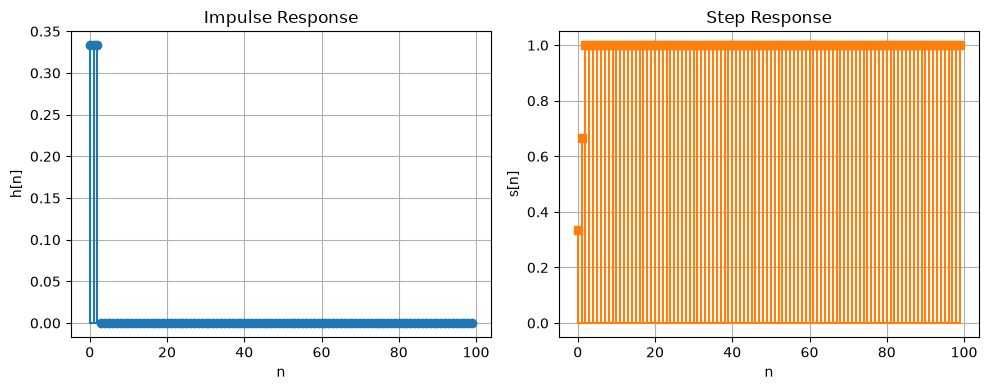
\includegraphics{3-point-moving-average.png}

\hypertarget{causal-first-order-iir}{%
\subsubsection{Causal First-Order IIR}\label{causal-first-order-iir}}

Determine \(h[n]\) of this system:

\[
y[n] = ay[n-1] + bx[n],
\quad \text{initial rest } (y[n] = 0 \text{ for } n < 0)
\]

\begin{enumerate}
\def\labelenumi{\arabic{enumi}.}
\item
  \textbf{Take the z-transform of both sides of the difference
  equation:}

  Applying the time-shifting property
  \(\mathcal{Z}\{y[n-1]\} = z^{-1} Y(z)\):

  \[Y(z) = a z^{-1} Y(z) + b X(z)\]
\item
  \textbf{Rearrange terms to form the system transfer function
  \(H(z) = \frac{Y(z)}{X(z)}\):}

  \[Y(z) - a z^{-1} Y(z) = b X(z)\]

  \[Y(z) (1 - a z^{-1}) = b X(z)\]

  \[H(z) = \frac{Y(z)}{X(z)} = \frac{b}{1 - a z^{-1}}\]
\item
  \textbf{Take the inverse z-transform (\(\mathcal{Z}^{-1}\)) of
  \(H(z)\):}

  Using the standard z-transform pair
  \(\mathcal{Z}^{-1}\left\{\frac{1}{1 - a z^{-1}}\right\} = a^n u[n]\)
  for a causal system:

  \[h[n] = \mathcal{Z}^{-1}\{H(z)\} = b \cdot \mathcal{Z}^{-1}\left\{\frac{1}{1 - a z^{-1}}\right\} = b a^n u[n]\]
\end{enumerate}

\textbf{Final Result}

\[h[n] = b a^n u[n]\]

\hypertarget{pole-zero-plot}{%
\subsubsection{Pole-Zero Plot}\label{pole-zero-plot}}

Sketch the pole-zero plot of this system:

\[
H(z) = \frac{1 - 0.5 z^-1}{1 - 0.7 z^-1 - z^-2}
\]

\begin{Shaded}
\begin{Highlighting}[]
\ImportTok{import}\NormalTok{ numpy }\ImportTok{as}\NormalTok{ np}
\ImportTok{import}\NormalTok{ matplotlib.pyplot }\ImportTok{as}\NormalTok{ plt}
\ImportTok{from}\NormalTok{ scipy }\ImportTok{import}\NormalTok{ signal}

\CommentTok{\# Example system: H(z) = (1 {-} 0.5 z\^{}{-}1) / (1 {-} 0.7 z\^{}{-}1 {-} z\^{}{-}2)}
\NormalTok{num }\OperatorTok{=}\NormalTok{ [}\DecValTok{1}\NormalTok{, }\OperatorTok{{-}}\FloatTok{0.5}\NormalTok{]}
\NormalTok{den }\OperatorTok{=}\NormalTok{ [}\DecValTok{1}\NormalTok{, }\OperatorTok{{-}}\FloatTok{0.7}\NormalTok{, }\OperatorTok{{-}}\DecValTok{1}\NormalTok{]}

\CommentTok{\# Get zeros, poles, gain}
\NormalTok{z, p, \_ }\OperatorTok{=}\NormalTok{ signal.tf2zpk(num, den) }\CommentTok{\# transfer to pole{-}zero plot}

\NormalTok{zeros\_r, zeros\_theta }\OperatorTok{=}\NormalTok{ np.}\BuiltInTok{abs}\NormalTok{(z), np.angle(z)}
\NormalTok{poles\_r, poles\_theta }\OperatorTok{=}\NormalTok{ np.}\BuiltInTok{abs}\NormalTok{(p), np.angle(p)}

\CommentTok{\# Draw unit circle}
\NormalTok{theta }\OperatorTok{=}\NormalTok{ np.linspace(}\DecValTok{0}\NormalTok{, }\DecValTok{2}\OperatorTok{*}\NormalTok{np.pi, }\DecValTok{400}\NormalTok{)}
\NormalTok{plt.polar(theta, np.ones\_like(theta), }\StringTok{\textquotesingle{}k{-}{-}\textquotesingle{}}\NormalTok{, linewidth}\OperatorTok{=}\DecValTok{1}\NormalTok{)}
\NormalTok{plt.polar(zeros\_theta, zeros\_r, }\StringTok{\textquotesingle{}bo\textquotesingle{}}\NormalTok{, label}\OperatorTok{=}\StringTok{"Zeros"}\NormalTok{)}
\NormalTok{plt.polar(poles\_theta, poles\_r, }\StringTok{\textquotesingle{}rx\textquotesingle{}}\NormalTok{, label}\OperatorTok{=}\StringTok{"Poles"}\NormalTok{)}
\NormalTok{plt.title(}\StringTok{"Pole{-}Zero Plot in Z{-}Domain"}\NormalTok{)}
\NormalTok{plt.legend(loc}\OperatorTok{=}\StringTok{"upper right"}\NormalTok{)}
\NormalTok{plt.show()}
\end{Highlighting}
\end{Shaded}

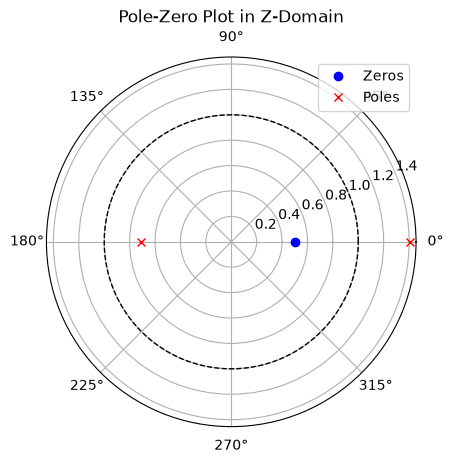
\includegraphics{pole-zero-plot.png}

\textbf{Remark}

This system is not BIBO stable as there exists a pole that lies outside
the unit circle.
